% Options for packages loaded elsewhere
\PassOptionsToPackage{unicode}{hyperref}
\PassOptionsToPackage{hyphens}{url}
%
\documentclass[
]{article}
\usepackage{amsmath,amssymb}
\usepackage{lmodern}
\usepackage{ifxetex,ifluatex}
\ifnum 0\ifxetex 1\fi\ifluatex 1\fi=0 % if pdftex
  \usepackage[T1]{fontenc}
  \usepackage[utf8]{inputenc}
  \usepackage{textcomp} % provide euro and other symbols
\else % if luatex or xetex
  \usepackage{unicode-math}
  \defaultfontfeatures{Scale=MatchLowercase}
  \defaultfontfeatures[\rmfamily]{Ligatures=TeX,Scale=1}
\fi
% Use upquote if available, for straight quotes in verbatim environments
\IfFileExists{upquote.sty}{\usepackage{upquote}}{}
\IfFileExists{microtype.sty}{% use microtype if available
  \usepackage[]{microtype}
  \UseMicrotypeSet[protrusion]{basicmath} % disable protrusion for tt fonts
}{}
\makeatletter
\@ifundefined{KOMAClassName}{% if non-KOMA class
  \IfFileExists{parskip.sty}{%
    \usepackage{parskip}
  }{% else
    \setlength{\parindent}{0pt}
    \setlength{\parskip}{6pt plus 2pt minus 1pt}}
}{% if KOMA class
  \KOMAoptions{parskip=half}}
\makeatother
\usepackage{xcolor}
\IfFileExists{xurl.sty}{\usepackage{xurl}}{} % add URL line breaks if available
\IfFileExists{bookmark.sty}{\usepackage{bookmark}}{\usepackage{hyperref}}
\hypersetup{
  pdftitle={O Método PDCA e Ferramentas da Qualidade},
  pdfauthor={Marcelo Carvalho},
  hidelinks,
  pdfcreator={LaTeX via pandoc}}
\urlstyle{same} % disable monospaced font for URLs
\usepackage[margin=1in]{geometry}
\usepackage{longtable,booktabs,array}
\usepackage{calc} % for calculating minipage widths
% Correct order of tables after \paragraph or \subparagraph
\usepackage{etoolbox}
\makeatletter
\patchcmd\longtable{\par}{\if@noskipsec\mbox{}\fi\par}{}{}
\makeatother
% Allow footnotes in longtable head/foot
\IfFileExists{footnotehyper.sty}{\usepackage{footnotehyper}}{\usepackage{footnote}}
\makesavenoteenv{longtable}
\usepackage{graphicx}
\makeatletter
\def\maxwidth{\ifdim\Gin@nat@width>\linewidth\linewidth\else\Gin@nat@width\fi}
\def\maxheight{\ifdim\Gin@nat@height>\textheight\textheight\else\Gin@nat@height\fi}
\makeatother
% Scale images if necessary, so that they will not overflow the page
% margins by default, and it is still possible to overwrite the defaults
% using explicit options in \includegraphics[width, height, ...]{}
\setkeys{Gin}{width=\maxwidth,height=\maxheight,keepaspectratio}
% Set default figure placement to htbp
\makeatletter
\def\fps@figure{htbp}
\makeatother
\setlength{\emergencystretch}{3em} % prevent overfull lines
\providecommand{\tightlist}{%
  \setlength{\itemsep}{0pt}\setlength{\parskip}{0pt}}
\setcounter{secnumdepth}{5}
\ifluatex
  \usepackage{selnolig}  % disable illegal ligatures
\fi

\title{O Método PDCA e Ferramentas da Qualidade}
\author{Marcelo Carvalho}
\date{2021-09-11}

\begin{document}
\maketitle

{
\setcounter{tocdepth}{2}
\tableofcontents
}
\hypertarget{preface}{%
\section*{Preface}\label{preface}}
\addcontentsline{toc}{section}{Preface}

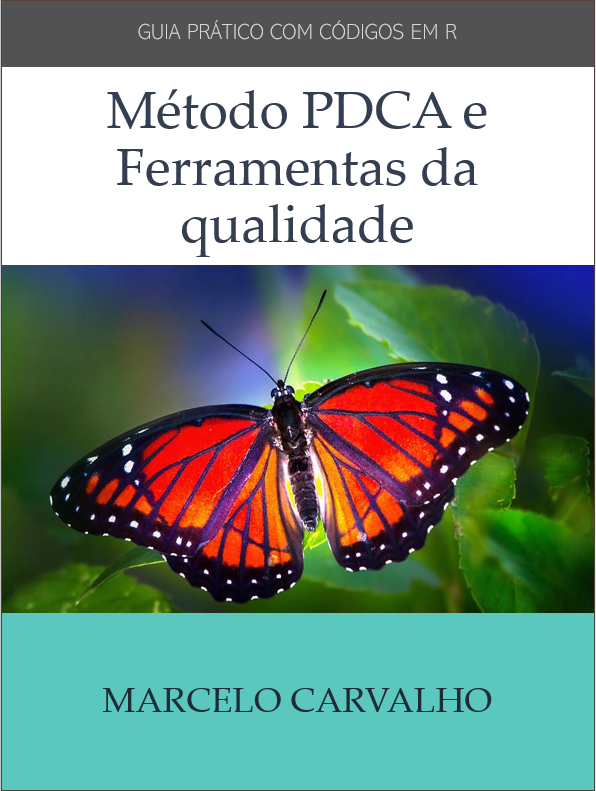
\includegraphics{images/pdca_capa.png}

O tema central do livro é a aplicação do método PDCA e ferramentas da qualidade e é uma etapa complementar de pesquisa de mestrado de 2010 na área do agronegócio onde foram adicionados elementos como mapas, desenhos, práticas de uso e código reproduzível.

Embora a pesquisa tenha sido feita no agronegócio, os conceitos abordados já foram testados, validados e usados em outras áreas ao longo do tempo por pesquisadores muito conhecidos no meio científico como Galileu Galilei, Da Vinci, Copérnico, Shewhart, Deming entre outros.

\hypertarget{introduuxe7uxe3o}{%
\section*{Introdução}\label{introduuxe7uxe3o}}
\addcontentsline{toc}{section}{Introdução}

Se trata de um livro técnico e para facilitar o entendimento dos temas abordados e das premissas que serão guias para coloboração, será organizado da seguinte forma:

\begin{itemize}
\tightlist
\item
  \textbf{O que é}: ou qual a ideia disso que esta sendo abordado.
\item
  \textbf{Qual o objetivo}: pra que isso está sendo, ou foi desenvolvido. Pode ter mais que um.
\item
  \textbf{De onde vem}: são as necessidades ou a origem dessa demanda ou etapa. A motivação.
\item
  \textbf{Como fazer}: é o procedimento, código, sequência ou fluxo. É importante que seja reproduzível.
\item
  \textbf{Pra onde vai}: é o destino. Quem é o consumidor ou qual a aplicação prática disso.
\item
  \textbf{Qual o resultado}: é a descrição dos resultados esperados, desejados ou comprovados.
\end{itemize}

\hypertarget{objetivo}{%
\subsection*{Objetivo}\label{objetivo}}
\addcontentsline{toc}{subsection}{Objetivo}

A ideia central desse trabalho é possibilitar que conceitos utilizados a algumas centenas de anos que foram testados novamente e validados 2010 possam ser usados na melhoria do desenvolvimento humano seja nos negócios, projetos pessoais ou comunitários dentro e fora do agronegócio. Para isso, alguns objetivos foram definidos:

\begin{itemize}
\item
  Facilitar o entendimento dos conceitos usando linguagem simples e exemplos práticos do dia a dia.
\item
  Permitir a replicação usando código reproduzível na linguagem de computação científica R.
\item
  Permitir a interação e compartilhamento de ideias e experiências. O leitor poderá sugerir, fazer alterações, adicionar complementos e ideias que enriqueça esse trabalho para todos.
\end{itemize}

\hypertarget{motivauxe7uxe3o}{%
\subsection*{Motivação}\label{motivauxe7uxe3o}}
\addcontentsline{toc}{subsection}{Motivação}

Em 2020, momento atual da história humana em que este livro está sendo escrito, 4 fenômenos estão sendo observados os quais podem se tornar desafiadores para todos os povos do planeta.

\begin{itemize}
\item
  \textbf{Transição demográfica} que descreve a mudança histórica de taxas de natalidade,mortalidade e crescimento populacional decorrentes do avanço da medicina, urbanização e desenvolvimento de novas técnologias. \textbf{Estamos ficando mais velhos} os idosos acima de 65 anos constituem a faixa etária de crescimento mais rápido do mundo. Algumas regiões como Europa e Ásia Oriental já enfrentam desafios para cuidar de sua população idosa.
  É provável que os idosos desempenhem papéis significativos nas sociedades e economias conforme a expectativa de vida aumenta. \textbf{Estamos ficando mais urbanos} em 2020 cerca de 55\% da população mundial vive em vilas e cidades. O acesso a economia e a sociedade digital em áreas ruais é um processo contínuo e pequenos agricultores, pastores e povos indígenas podem desempenhar papel vital na produção de alimentos e na proteção do meio ambiente.
\item
  \textbf{Tecnolodias disrruptivas} instrumentos e técnicas que potencializam as capacidades humanas como inteligência artificial, veículos autonomos, blockchain, impressão 3D, realidade virtual e aumentada, internet das coisas e edição genética CRISPR estão sendo aprimorados e podem modificar substancialmente o modo como as coisas são feitas.
\item
  \textbf{Atividade economica em países emergentes} em 2020 países como Indonésia, Africa do Sul, Russia, México, Malasia, Colombia, Polônia, Chile, Hingria, Tailandia, Turquia, Brasil, China e Índia são considerandos países emergentes. Boa parte desses países, têm feito progressos notáveis no fortalecimento de seus políticas macroeconômicas desde a virada do século o que os permitiu mais do que dobrar a renda per capita em média.
\item
  \textbf{Mudanças climáticas} impactam diretamente no comportamento das pessoas o que reflete diretamente na demanda, consequentemente nos meios de produção o que também altera a forma como as coisas são feitas.
\end{itemize}

\hypertarget{desafios-da-agroindustria}{%
\subsection*{Desafios da Agroindustria}\label{desafios-da-agroindustria}}
\addcontentsline{toc}{subsection}{Desafios da Agroindustria}

\begin{itemize}
\item
  \textbf{Na perspectiva de demanda} necessidades cada vez maiores de produtos(volume e variedade), exigência por qualidade, segurança, cuidado com o meio ambiente e com as comunidades também são demandas crescentes.
\item
  \textbf{Na perspectiva de produção} necessidade de melhorias nas práticas de cultivo para lidar com trade-off entre aumento de demanda e restrições de área, outros fatores como ganhos de produtivide, eficiência no aproveitamente de recursos e redução de desperdícios e perdas pode se tornar variáveis mais importantes na competitividade global.
\end{itemize}

\hypertarget{conceitos}{%
\section{Conceitos}\label{conceitos}}

\hypertarget{muxe9todo-pdca}{%
\subsection{Método PDCA}\label{muxe9todo-pdca}}

O PDCA é um método criado para auxiliar os gestores na identificação e solução de problemas. Ele mostra de forma simplificada e organizada o caminho a ser percorrido na busca de melhoria contínua.

Também conhecido como ciclo de Shewhart ou ciclo de Deming, foi concluído em 1930 por Walter Shewhart no Bell Laboratories, que, analisando estatisticamente o controle de processos, criou um modelo que poderia ser aplicado em qualquer situação (WERKEMA, 1995).

O estatístico norte americano William Edwards Deming foi o responsável por propagar a idéia no Japão após a segunda guerra mundial. Desde então, obteve-se a popularização ao redor do mundo, das técnicas e da qualidade dos produtos japoneses, os quais antes da guerra competiam no mercado internacional apenas em preço e não em qualidade.

Segundo Campos (1995), o ciclo PDCA tem por princípio tornar mais claras e ágeis as etapas no processo de gerenciamento as quais são assim divididas:

\begin{itemize}
\item
  \textbf{PLAN (Planejamento)} - Etapa que tem por objetivo, identificar oportunidades ou problemas, analisar os fenômenos e causas reais, estabelecer metas e determinar os procedimentos necessários para o cumprimento desses nos prazos estabelecidos.
\item
  \textbf{DO (Execução)} - Realizar ou executar as ações propostas na etapa anterior ou \textbf{Plan}, por meio da busca pelo aprendizado.
\item
  \textbf{CHECK (Verificação)} -- É a etapa en que são realizados as avaliações, o monitoramento e o controle das ações que estão sendo executadas, comparando-se os resultados com o que foi planejado na etapa \textbf{Plan}.
\item
  \textbf{ACT (Ação e padronização)} - Etapa de validação dos resultados os quais poderão ser adotados como padrão caso o objetivo tenha sido alcançado.
\end{itemize}

\begin{figure}
\centering
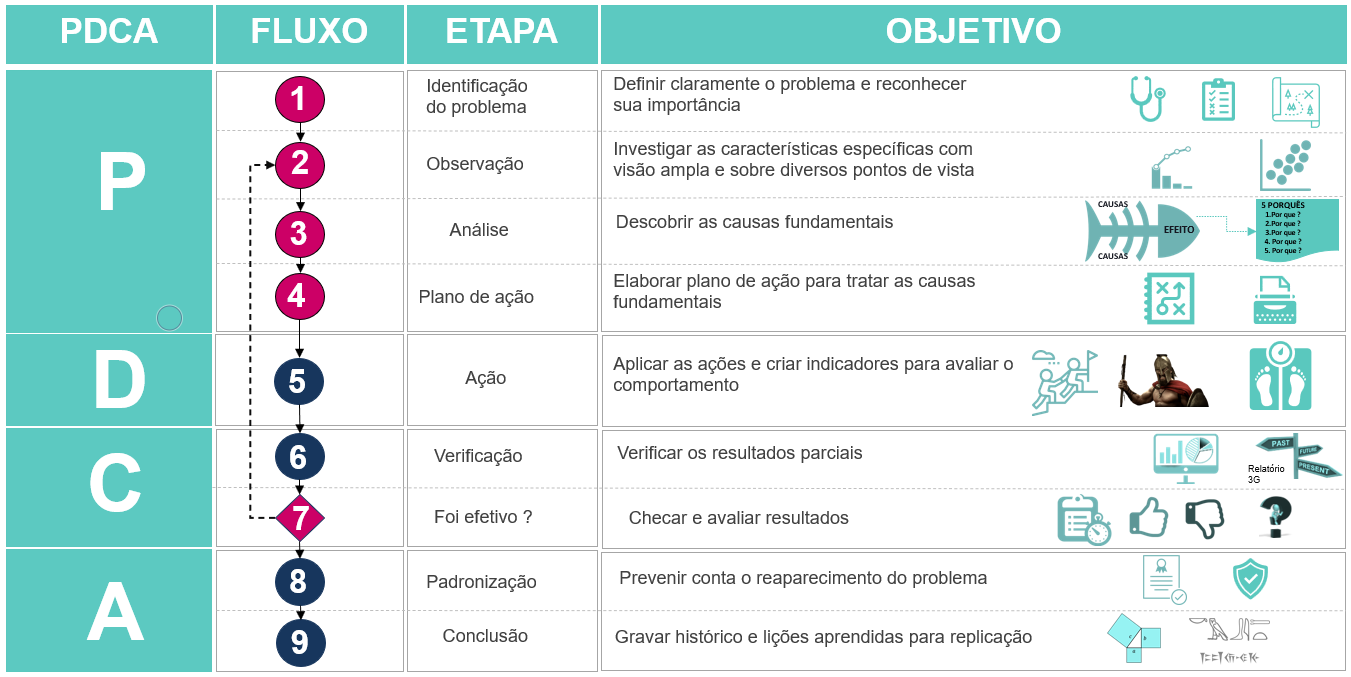
\includegraphics{images/pdca_chart.png}
\caption{Figura 1 - Ilustração médoto PDCA}
\end{figure}

\hypertarget{ferramentas-da-qualidade}{%
\subsection{Ferramentas da qualidade}\label{ferramentas-da-qualidade}}

As ferramentas da qualidade modernas foram descobertas na década de 1930 nos Estados Unidos, com a aplicação industrial do gráfico de controle criado por Walter Shewhart da empresa de telefonia Bell Telephone Laboratories.

Shewhart, que propôs um gráfico de controle para análise de dados resultantes de inspeção, fazendo com que a importância dada a procedimentos de inspeção e correção de produtos defeituosos começasse a ser substituída por estudos e prevenção dos problemas relacionados à qualidade, de modo a garantir que o possível defeito do produto fosse eliminado durante o processo e não após o término (FERRO, 1997).

Após a segunda guerra mundial, o Japão em especial, passou por uma verdadeira revolução, onde a qualidade dos produtos e serviços nunca foi tão discutida, estudada e aplicada. Grandes nomes como Shewhart, Deming, Juran e Ishikawa, desenvolveram ou ajudaram a disseminar algumas ferramentas que permitiram um maior controle dos processos ou melhoria nas tomadas de decisões (CAMPOS, 1995).

Nas décadas de 1970 e 1980, essas técnicas e ferramentas começaram a ser introduzidas em empresas de diversos países da Ásia, Europa, América do Norte e América Latina, influenciados principalmente pela maior competitividade dos produtos japoneses por meio de alta qualidade e preços competitivos (FERRO, 1997).

No Brasil, o uso de ferramentas da qualidade na gestão de empresas ocorreu por volta de 1970, sendo introduzido em algumas empresas como Volkswagen, Johnson \& Johnson e Embraer, tendo seu movimento impulsionado em 1986, quando o professor Ishikawa esteve no país.

\hypertarget{fluxograma-de-processos}{%
\section{Fluxograma de Processos}\label{fluxograma-de-processos}}

\hypertarget{o-que-uxe9}{%
\subsection*{O que é}\label{o-que-uxe9}}
\addcontentsline{toc}{subsection}{O que é}

\hypertarget{qual-o-objetivo}{%
\subsection*{Qual o objetivo}\label{qual-o-objetivo}}
\addcontentsline{toc}{subsection}{Qual o objetivo}

\begin{itemize}
\tightlist
\item
  A
\item
  B
\item
  C
\end{itemize}

\hypertarget{de-onde-vem}{%
\subsection*{De onde vem}\label{de-onde-vem}}
\addcontentsline{toc}{subsection}{De onde vem}

\begin{itemize}
\tightlist
\item
  A
\item
  B
\item
  C
\end{itemize}

\hypertarget{como-fazer}{%
\subsection*{Como fazer}\label{como-fazer}}
\addcontentsline{toc}{subsection}{Como fazer}

\begin{itemize}
\tightlist
\item
  A
\item
  B
\item
  C
\end{itemize}

\hypertarget{pra-onde-vai}{%
\subsection*{Pra onde vai}\label{pra-onde-vai}}
\addcontentsline{toc}{subsection}{Pra onde vai}

\begin{itemize}
\tightlist
\item
  A
\item
  B
\item
  C
\end{itemize}

\hypertarget{qual-o-resultado}{%
\subsection*{Qual o resultado}\label{qual-o-resultado}}
\addcontentsline{toc}{subsection}{Qual o resultado}

\begin{itemize}
\tightlist
\item
  A
\item
  B
\item
  C
\end{itemize}

O fluxograma é uma representação gráfica das etapas de um processo e a relação entre elas. É bastante utilizado para entender um processo e identificar as oportunidades de melhoria, facilitar a comunicação entre as pessoas envolvidas no processo e disseminar informações. Além da sequência de atividades, o fluxograma mostra o que é realizado em cada etapa, materiais e serviços que entram e saem do processo, decisões que devem ser tomadas e também as pessoas envolvidas. Utiliza símbolos que são reconhecidos facilmente para representar cada etapa, pessoas ou setores envolvidos no processo (BRASSARD, 1994).

Existem vários tipos de fluxogramas, no entanto, o mais utilizado é o fluxograma de bloco. Os símbolos mais comuns utilizados na montagem de um fluxograma de bloco são:

\begin{itemize}
\item
  \textbf{Limites}: representado por figura em formato de elipse indica o início e o fim do processo.
\item
  \textbf{Operação}: é representada por um retângulo, e sinaliza uma etapa do processo ou atividade. O nome da etapa e quem a executa são registrados no interior do retângulo.
\item
  \textbf{Decisão}: é representado por um losango e indica um ponto em que alguma decisão deve ser tomada. Duas setas saindo do losango mostram a direção do processo em função da resposta que geralmente é SIM ou NÃO.
\item
  \textbf{Sentido fluxo}: representado por uma linha com seta e indica o sentido e a sequência do processo.
\end{itemize}

O fluxograma pode ser utilizado em vários estudos, como mapeamento de processos de produção, percurso de uma fatura, fases de uma operação de venda, fluxo de matérias entre outras aplicações.

\hypertarget{folha-de-verificauxe7uxe3o-check-list}{%
\section{Folha de verificação (Check-list)}\label{folha-de-verificauxe7uxe3o-check-list}}

\hypertarget{o-que-uxe9-1}{%
\subsection*{O que é}\label{o-que-uxe9-1}}
\addcontentsline{toc}{subsection}{O que é}

A folha de verificação, check sheet ou check list como também é conhecida, trata-se de um formulário impresso ou por meio digital. É uma ferramenta bastante simples utilizada para a coleta de dados quantitativos e qualitativos em tempo real no local onde os dados são gerados. O objetivo principal da folha de verificação é a coleta de dados de forma estruturada e organizada, dispondo de dados autoexplicativos e que são rapidamente vistos e interpretados corretamente por todos (KUME, 1993).

\hypertarget{qual-o-objetivo-1}{%
\subsection*{Qual o objetivo}\label{qual-o-objetivo-1}}
\addcontentsline{toc}{subsection}{Qual o objetivo}

Alguns benefícios do uso da folha de verificação na coleta de dados é a economia de tempo, pois elimina a necessidade de desenhar figuras ou escrever números repetitivos, e evita também que problemas como falhas na interpretação comprometam o tratamento e análise dos dados, principalmente em situações em que várias pessoas participam da etapa de coleta (WERKEMA, 1995).

\hypertarget{de-onde-vem-1}{%
\subsection*{De onde vem}\label{de-onde-vem-1}}
\addcontentsline{toc}{subsection}{De onde vem}

Algumas características são comuns em uma folha de verificação, como a indicação dos itens que serão verificados, o período, o motivo e a frequência. Essa folha, relaciona-se com quase todas as demais ferramentas estatísticas, pois é a etapa inicial e onde se encontram os dados que serão analisados (WERKEMA, 1995).

\hypertarget{como-fazer-1}{%
\subsection*{Como fazer}\label{como-fazer-1}}
\addcontentsline{toc}{subsection}{Como fazer}

Segundo Kume (1993), existem alguns preceitos básicos na elaboração de uma folha de verificação, que é o agrupamento de elementos com características semelhantes tendo causa e soluções comuns, além de dividi-los em algumas categorias:

\begin{itemize}
\item
  folha de verificação para distribuição de processos de produção: coleta-se os dados de amostras de produção para se calcular a variação do processo produtivo;
\item
  folha de verificação para produtos defeituosos: coletam-se os dados para identificar os defeitos mais frequêntes, bem como o número de vezes de cada motivo;
\item
  folhas de verificação para localizar os defeitos: a coleta de dados geralmente é composta de um desenho, figura ou mapa do item a ser verificado no qual são assinalados o local e a forma da ocorrência dos defeitos;
\item
  folha de verificação de causa e defeitos: coleta de dados em que os dados relativos às causas e aos defeitos são dispostos de forma ordenada, tornando muito clara a relação entre eles.
  Brassard (1994), observa que as folhas de verificação (Figura 7), por serem uma ferramenta de fácil compreensão e fácil elaboração, são utilizadas na coleta de dados amostrais com o objetivo de se formar um modelo. É o ponto lógico de início na maioria dos ciclos de solução de problemas.
\end{itemize}

\hypertarget{pra-onde-vai-1}{%
\subsection*{Pra onde vai}\label{pra-onde-vai-1}}
\addcontentsline{toc}{subsection}{Pra onde vai}

\hypertarget{qual-o-resultado-1}{%
\subsection*{Qual o resultado}\label{qual-o-resultado-1}}
\addcontentsline{toc}{subsection}{Qual o resultado}

\hypertarget{gruxe1fico-de-disperuxe7uxe3o}{%
\section{Gráfico de Disperção}\label{gruxe1fico-de-disperuxe7uxe3o}}

\hypertarget{o-que-uxe9-2}{%
\subsection*{O que é}\label{o-que-uxe9-2}}
\addcontentsline{toc}{subsection}{O que é}

\hypertarget{qual-o-objetivo-2}{%
\subsection*{Qual o objetivo}\label{qual-o-objetivo-2}}
\addcontentsline{toc}{subsection}{Qual o objetivo}

\begin{itemize}
\tightlist
\item
  A
\item
  B
\item
  C
\end{itemize}

\hypertarget{de-onde-vem-2}{%
\subsection*{De onde vem}\label{de-onde-vem-2}}
\addcontentsline{toc}{subsection}{De onde vem}

\begin{itemize}
\tightlist
\item
  A
\item
  B
\item
  C
\end{itemize}

\hypertarget{como-fazer-2}{%
\subsection*{Como fazer}\label{como-fazer-2}}
\addcontentsline{toc}{subsection}{Como fazer}

\begin{itemize}
\tightlist
\item
  A
\item
  B
\item
  C
\end{itemize}

\hypertarget{pra-onde-vai-2}{%
\subsection*{Pra onde vai}\label{pra-onde-vai-2}}
\addcontentsline{toc}{subsection}{Pra onde vai}

\begin{itemize}
\tightlist
\item
  A
\item
  B
\item
  C
\end{itemize}

\hypertarget{qual-o-resultado-2}{%
\subsection*{Qual o resultado}\label{qual-o-resultado-2}}
\addcontentsline{toc}{subsection}{Qual o resultado}

\begin{itemize}
\tightlist
\item
  A
\item
  B
\item
  C
\end{itemize}

O gráfico de Pareto, é uma ferramenta que tem como objetivo principal identificar quais causas seriam responsáveis pela maior parcela dos efeitos.

Sua origem decorre de estudos do economista italiano Vilfredo Pareto, no qual ele afirma que para muitos fenômenos, 80\% das consequências advêm de 20\% das causas. Esses estudos foram aprofundados por Joseph Moses Juran, o qual expandiu essa lei para a esfera organizacional nos Estados Unidos a partir da década de 1930 (BRASSARD, 1994).

O gráfico de Pareto, também conhecido como diagrama 80/20, é um tipo específico de histograma ordenado por frequência de ocorrência da maior para a menor, permitindo assim a priorização das ações partindo-se do princípio de Pareto, de que há muitos efeitos sem importância diante de outros mais graves (BRASSARD, 1994).

Mesmo como priorização dos efeitos com maior número de ocorrências apresentados no gráfico de Pareto, os demais também são importantes e não devem ser descartados ou ignorados, pois contrariam a teoria da confiabilidade de Russel, a qual defende que mesmo os problemas de pequenas proporções quando somados a outros da mesma dimensão, resultam em um conjunto com confiabilidade bastante reduzida (NAKATA, 2000).

\hypertarget{diagrama-de-causa-e-efeitoishikawa}{%
\section{Diagrama de Causa e Efeito(Ishikawa)}\label{diagrama-de-causa-e-efeitoishikawa}}

\hypertarget{o-que-uxe9-3}{%
\subsection*{O que é}\label{o-que-uxe9-3}}
\addcontentsline{toc}{subsection}{O que é}

\hypertarget{qual-o-objetivo-3}{%
\subsection*{Qual o objetivo}\label{qual-o-objetivo-3}}
\addcontentsline{toc}{subsection}{Qual o objetivo}

\begin{itemize}
\tightlist
\item
  A
\item
  B
\item
  C
\end{itemize}

\hypertarget{de-onde-vem-3}{%
\subsection*{De onde vem}\label{de-onde-vem-3}}
\addcontentsline{toc}{subsection}{De onde vem}

\begin{itemize}
\tightlist
\item
  A
\item
  B
\item
  C
\end{itemize}

\hypertarget{como-fazer-3}{%
\subsection*{Como fazer}\label{como-fazer-3}}
\addcontentsline{toc}{subsection}{Como fazer}

\begin{itemize}
\tightlist
\item
  A
\item
  B
\item
  C
\end{itemize}

\hypertarget{pra-onde-vai-3}{%
\subsection*{Pra onde vai}\label{pra-onde-vai-3}}
\addcontentsline{toc}{subsection}{Pra onde vai}

\begin{itemize}
\tightlist
\item
  A
\item
  B
\item
  C
\end{itemize}

\hypertarget{qual-o-resultado-3}{%
\subsection*{Qual o resultado}\label{qual-o-resultado-3}}
\addcontentsline{toc}{subsection}{Qual o resultado}

\begin{itemize}
\tightlist
\item
  A
\item
  B
\item
  C
\end{itemize}

O diagrama de causa e efeito, também conhecido como diagrama de Ishikawa ou espinha de peixe, é uma ferramenta gráfica utilizada no gerenciamento de diversos processos e de diversos projetos. Originalmente, proposto pelo engenheiro químico japonês Kaoru Ishikawa em 1943, e aperfeiçoado nos anos seguintes, o diagrama de Ishikawa (Figura 5) permite que seja identificada uma relação significativa entre o efeito e suas possíveis causas (WERKEMA, 1995).

Essa ferramenta foi utilizada pela primeira vez no Japão por volta de 1953, com o objetivo de sintetizar as opiniões dos engenheiros de uma fábrica quando estes discutem problemas referentes à qualidade dos produtos (SEBRAE, 2009),

Esse sistema permite estruturar hierarquicamente as causas de determinado problema ou oportunidade de melhoria, bem como seus efeitos sobre a qualidade dos produtos. Permite também, estruturar qualquer sistema que necessite de resposta de forma gráfica e sintética, obtendo melhor visualização (SEBRAE, 2009).

\hypertarget{gruxe1fico-de-pareto}{%
\section{Gráfico de Pareto}\label{gruxe1fico-de-pareto}}

\hypertarget{o-que-uxe9-4}{%
\subsection*{O que é}\label{o-que-uxe9-4}}
\addcontentsline{toc}{subsection}{O que é}

\hypertarget{qual-o-objetivo-4}{%
\subsection*{Qual o objetivo}\label{qual-o-objetivo-4}}
\addcontentsline{toc}{subsection}{Qual o objetivo}

\begin{itemize}
\tightlist
\item
  A
\item
  B
\item
  C
\end{itemize}

\hypertarget{de-onde-vem-4}{%
\subsection*{De onde vem}\label{de-onde-vem-4}}
\addcontentsline{toc}{subsection}{De onde vem}

\begin{itemize}
\tightlist
\item
  A
\item
  B
\item
  C
\end{itemize}

\hypertarget{como-fazer-4}{%
\subsection*{Como fazer}\label{como-fazer-4}}
\addcontentsline{toc}{subsection}{Como fazer}

\begin{itemize}
\tightlist
\item
  A
\item
  B
\item
  C
\end{itemize}

\hypertarget{pra-onde-vai-4}{%
\subsection*{Pra onde vai}\label{pra-onde-vai-4}}
\addcontentsline{toc}{subsection}{Pra onde vai}

\begin{itemize}
\tightlist
\item
  A
\item
  B
\item
  C
\end{itemize}

\hypertarget{qual-o-resultado-4}{%
\subsection*{Qual o resultado}\label{qual-o-resultado-4}}
\addcontentsline{toc}{subsection}{Qual o resultado}

\begin{itemize}
\tightlist
\item
  A
\item
  B
\item
  C
\end{itemize}

O gráfico de Pareto, é uma ferramenta que tem como objetivo principal identificar quais causas seriam responsáveis pela maior parcela dos efeitos.

Sua origem decorre de estudos do economista italiano Vilfredo Pareto, no qual ele afirma que para muitos fenômenos, 80\% das consequências advêm de 20\% das causas. Esses estudos foram aprofundados por Joseph Moses Juran, o qual expandiu essa lei para a esfera organizacional nos Estados Unidos a partir da década de 1930 (BRASSARD, 1994).

O gráfico de Pareto, também conhecido como diagrama 80/20, é um tipo específico de histograma ordenado por frequência de ocorrência da maior para a menor, permitindo assim a priorização das ações partindo-se do princípio de Pareto, de que há muitos efeitos sem importância diante de outros mais graves (BRASSARD, 1994).

Mesmo como priorização dos efeitos com maior número de ocorrências apresentados no gráfico de Pareto, os demais também são importantes e não devem ser descartados ou ignorados, pois contrariam a teoria da confiabilidade de Russel, a qual defende que mesmo os problemas de pequenas proporções quando somados a outros da mesma dimensão, resultam em um conjunto com confiabilidade bastante reduzida (NAKATA, 2000).

\hypertarget{muxe9todo-5-porquuxeas}{%
\section{Método 5 porquês}\label{muxe9todo-5-porquuxeas}}

\hypertarget{o-que-uxe9-5}{%
\subsection*{O que é}\label{o-que-uxe9-5}}
\addcontentsline{toc}{subsection}{O que é}

\hypertarget{qual-o-objetivo-5}{%
\subsection*{Qual o objetivo}\label{qual-o-objetivo-5}}
\addcontentsline{toc}{subsection}{Qual o objetivo}

\begin{itemize}
\tightlist
\item
  A
\item
  B
\item
  C
\end{itemize}

\hypertarget{de-onde-vem-5}{%
\subsection*{De onde vem}\label{de-onde-vem-5}}
\addcontentsline{toc}{subsection}{De onde vem}

\begin{itemize}
\tightlist
\item
  A
\item
  B
\item
  C
\end{itemize}

\hypertarget{como-fazer-5}{%
\subsection*{Como fazer}\label{como-fazer-5}}
\addcontentsline{toc}{subsection}{Como fazer}

\begin{itemize}
\tightlist
\item
  A
\item
  B
\item
  C
\end{itemize}

\hypertarget{pra-onde-vai-5}{%
\subsection*{Pra onde vai}\label{pra-onde-vai-5}}
\addcontentsline{toc}{subsection}{Pra onde vai}

\begin{itemize}
\tightlist
\item
  A
\item
  B
\item
  C
\end{itemize}

\hypertarget{qual-o-resultado-5}{%
\subsection*{Qual o resultado}\label{qual-o-resultado-5}}
\addcontentsline{toc}{subsection}{Qual o resultado}

\begin{itemize}
\tightlist
\item
  A
\item
  B
\item
  C
\end{itemize}

Os cinco porquês é uma técnica desenvolvida no Japão por Sakichi Toyoda fundador da Toyota. A utilização é bastante simples e consiste em perguntar: Por que o fato ocorreu? Para a resposta, perguntar ``por quê?'' novamente, e assim seguir até encontrar o motivo real, a causa raiz. Não são necessárias exatamente cinco interações, podem ser menos ou mais. O objetivo principal da técnica é realmente encontrar a causa raiz do problema, evitando tomar ações paliativas (MERIGHI, 2009).

Merighi (2009) afirma que embora a ferramenta dos cinco porquês seja utilizada com grande frequência quando se procura encontrar a causa raiz de um determinado problema, em algumas situações a resposta ao ``por quê?'', nem sempre é suficiente para explicar a causa anterior analisada, pois a origem do problema pode partir de diferentes causas ou um conjunto delas, o que a torna mais complexa, sendo necessário fazer uma associação de causa e efeito.

\hypertarget{gruxe1fico-de-controle}{%
\section{Gráfico de controle}\label{gruxe1fico-de-controle}}

\hypertarget{o-que-uxe9-6}{%
\subsection*{O que é}\label{o-que-uxe9-6}}
\addcontentsline{toc}{subsection}{O que é}

\hypertarget{qual-o-objetivo-6}{%
\subsection*{Qual o objetivo}\label{qual-o-objetivo-6}}
\addcontentsline{toc}{subsection}{Qual o objetivo}

\begin{itemize}
\tightlist
\item
  A
\item
  B
\item
  C
\end{itemize}

\hypertarget{de-onde-vem-6}{%
\subsection*{De onde vem}\label{de-onde-vem-6}}
\addcontentsline{toc}{subsection}{De onde vem}

\begin{itemize}
\tightlist
\item
  A
\item
  B
\item
  C
\end{itemize}

\hypertarget{como-fazer-6}{%
\subsection*{Como fazer}\label{como-fazer-6}}
\addcontentsline{toc}{subsection}{Como fazer}

\begin{itemize}
\tightlist
\item
  A
\item
  B
\item
  C
\end{itemize}

\hypertarget{pra-onde-vai-6}{%
\subsection*{Pra onde vai}\label{pra-onde-vai-6}}
\addcontentsline{toc}{subsection}{Pra onde vai}

\begin{itemize}
\tightlist
\item
  A
\item
  B
\item
  C
\end{itemize}

\hypertarget{qual-o-resultado-6}{%
\subsection*{Qual o resultado}\label{qual-o-resultado-6}}
\addcontentsline{toc}{subsection}{Qual o resultado}

\begin{itemize}
\tightlist
\item
  A
\item
  B
\item
  C
\end{itemize}

O gráfico de controle ou carta de controle como também é conhecido, é uma ferramenta gráfica criada pelo estatístico americano Walter Andrew Shewhart em 1924 como um método de analisar e ajustar variações de um processo em função do tempo.

Duas características fundamentais descreviam os processos: centralização, que era determinada pela média representada por limite de controle (LC), e dispersão, que era determinada pelo desvio-padrão ou amplitude.

O desvio-padrão nos gráficos de controle, é representado por linhas paralelas em relação à média, as quais são chamadas de limites de controle, sendo, limite superior de controle (LSC), que é a linha superior à média, e limite inferior de controle (LIC), que é a linha inferior à média e não pode ser menor que zero. Um valor comum utilizado no estabelecimento de limites em um gráfico de controle é e pode ser justificado pelos bons resultados obtidos na prática, com o nível de confiança estabelecido de 99,74\% na análise dos dados (BRASSARD, 1994).

Em algumas situações particulares, os limites de controle poderão ser ajustados, por exemplo, aumentar o limite para quando os custos de investigação das causas forem muito grandes e reduzir para quando as análises das possíveis causas do surgimento de fatores especiais de variação forem simples, consumirem o mínimo de tempo, e em situações em que o custo de produção de artigos defeituosos for alto (DEMING, 2003).

Os gráficos de controle são divididos em dois grupos: de controle por variáveis e por atributos. O gráfico de controle por variáveis é formado por dados quantitativos, mensuráveis ou que variam continuamente, e é utilizado quando as amostras são expressas em unidades quantitativas de medida tais como comprimento, largura, peso, tempo. O mais comum desses gráficos é o Xbarra-R ou , onde se determinam a média e amplitude das amostras de cada grupo (VIEIRA e WADA,1992).

O gráfico de controle por atributos é representado por dados que só podem ser contados ou classificados e é utilizado quando as amostras refletem características qualitativas como defeituoso ou não, passa ou não passa, entre outros. Para esse tipo de controle é comumente utilizado o gráfico P, NP, C e U, os quais serão apresentados nos apêncides B, C, D, E. Os gráficos de controle por atributos são utilizados geralmente quando a medição da característica é inviável, antieconômica ou há conveniência em transformar uma variável em atributo; no entanto, é importante acrescentar que uma variável transmite mais informação do que atributos (BRASSARD, 1994).

Os gráficos P e NP são utilizados quando os atributos são do tipo classificação, por exemplo, SIM ou NÃO, PASSA ou NÃO PASSA, onde em classificações com tamanhos de amostra variável, é mais indicado o gráfico P.
Os limites de controle para o gráfico P, de fração defeituosa total na
amostra, são:

Deming (1997), descreve que Shewhart descobriu duas formas de variações em um processo as quais ele classificou como causas comuns, as quais afetam todos os valores individuais do resultado do processo mas que se enquadram dentro dos limites de controle e representam um processo estável, e as causas especiais, que compreendem as variações intermitentes, imprevisíveis ou instáveis, e são sinalizadas de várias formas, como um ponto fora dos limites de controle, ausência de padrões não aleatórios ou tendências dentro do limite de controle (Figura 10).

Uma das dificuldades das empresas ao trabalhar com gráficos de controle, é diferenciar as causas que geraram o problema, se são comuns ou especiais, no entanto, existem diferenças em alguns aspectos. As causas especiais geralmente apresentam pequenas perdas monetárias, grandes visibilidades do problema por causa da variação súbita, facilidade na coleta e análise dos dados e a responsabilidade para as ações de restabelecer o nível anterior fica por conta do pessoal envolvido no processo.

Nas causas comuns, as características são bem diferentes pois apresentam na maioria das vezes, grandes perdas monetárias, a visibilidade do problema se torna difícil por causa da natureza contínua, a coleta e análise dos dados se tornam complexas e devem ser realizadas por equipe técnica cuja responsabilidade para as ações fica por conta da administração, pois se trata de mudanças no sistema ou projeto (DEMING, 2003).

\hypertarget{plano-de-auxe7uxe3o}{%
\section{Plano de Ação}\label{plano-de-auxe7uxe3o}}

\hypertarget{o-que-uxe9-7}{%
\subsection*{O que é}\label{o-que-uxe9-7}}
\addcontentsline{toc}{subsection}{O que é}

\hypertarget{qual-o-objetivo-7}{%
\subsection*{Qual o objetivo}\label{qual-o-objetivo-7}}
\addcontentsline{toc}{subsection}{Qual o objetivo}

\begin{itemize}
\tightlist
\item
  A
\item
  B
\item
  C
\end{itemize}

\hypertarget{de-onde-vem-7}{%
\subsection*{De onde vem}\label{de-onde-vem-7}}
\addcontentsline{toc}{subsection}{De onde vem}

\begin{itemize}
\tightlist
\item
  A
\item
  B
\item
  C
\end{itemize}

\hypertarget{como-fazer-7}{%
\subsection*{Como fazer}\label{como-fazer-7}}
\addcontentsline{toc}{subsection}{Como fazer}

\begin{itemize}
\tightlist
\item
  A
\item
  B
\item
  C
\end{itemize}

\hypertarget{pra-onde-vai-7}{%
\subsection*{Pra onde vai}\label{pra-onde-vai-7}}
\addcontentsline{toc}{subsection}{Pra onde vai}

\begin{itemize}
\tightlist
\item
  A
\item
  B
\item
  C
\end{itemize}

\hypertarget{qual-o-resultado-7}{%
\subsection*{Qual o resultado}\label{qual-o-resultado-7}}
\addcontentsline{toc}{subsection}{Qual o resultado}

\begin{itemize}
\tightlist
\item
  A
\item
  B
\item
  C
\end{itemize}

O plano de ação ou 5W2H é uma ferramenta utilizada para detalhar e organizar todas as tarefas a serem executadas para a resolução do problema, assegurando a sua implementação efetiva, e é considerada a etapa principal do ciclo PDCA, onde as ações são implementadas (CAMPOS, 1994).

O nome 5W2H surgiu do conjunto das primeiras letras (em inglês) das diretrizes utilizadas no plano de ação, sendo cinco delas iniciadas em ``W'' e duas delas em ``H'', e são classificadas em:

\begin{itemize}
\tightlist
\item
  \textbf{What} -- O que será feito (etapas);
\item
  \textbf{Who} -- Quem o fará (responsabilidade);
\item
  \textbf{When} -- Quando será feito (tempo);
\item
  \textbf{Where} -- Onde será feito (local);
\item
  \textbf{Why} -- Por que será feito (justificativa);
\item
  \textbf{How} -- Como será feito (método);
\item
  \textbf{How much} -- Quanto custará para ser feito (custo).
\end{itemize}

O plano de ação (Figura 11), após serem definidas todas essas etapas, deve ficar em local visível por toda a equipe para que as ações passem a ser executadas efetivamente

\hypertarget{relatuxf3rio-de-truxeas-gerauxe7uxf5es}{%
\section{Relatório de três gerações}\label{relatuxf3rio-de-truxeas-gerauxe7uxf5es}}

\hypertarget{o-que-uxe9-8}{%
\subsection*{O que é}\label{o-que-uxe9-8}}
\addcontentsline{toc}{subsection}{O que é}

\hypertarget{qual-o-objetivo-8}{%
\subsection*{Qual o objetivo}\label{qual-o-objetivo-8}}
\addcontentsline{toc}{subsection}{Qual o objetivo}

\begin{itemize}
\tightlist
\item
  A
\item
  B
\item
  C
\end{itemize}

\hypertarget{de-onde-vem-8}{%
\subsection*{De onde vem}\label{de-onde-vem-8}}
\addcontentsline{toc}{subsection}{De onde vem}

\begin{itemize}
\tightlist
\item
  A
\item
  B
\item
  C
\end{itemize}

\hypertarget{como-fazer-8}{%
\subsection*{Como fazer}\label{como-fazer-8}}
\addcontentsline{toc}{subsection}{Como fazer}

\begin{itemize}
\tightlist
\item
  A
\item
  B
\item
  C
\end{itemize}

\hypertarget{pra-onde-vai-8}{%
\subsection*{Pra onde vai}\label{pra-onde-vai-8}}
\addcontentsline{toc}{subsection}{Pra onde vai}

\begin{itemize}
\tightlist
\item
  A
\item
  B
\item
  C
\end{itemize}

\hypertarget{qual-o-resultado-8}{%
\subsection*{Qual o resultado}\label{qual-o-resultado-8}}
\addcontentsline{toc}{subsection}{Qual o resultado}

\begin{itemize}
\tightlist
\item
  A
\item
  B
\item
  C
\end{itemize}

O relatório de três gerações é uma ferramenta que apresenta os dados agrupados e ordenados de acordo com três fases temporais de um determinado problema, que está sendo tratado:

\begin{itemize}
\item
  \textbf{Passado} -- o que foi planejado e o que foi feito.
\item
  \textbf{Presente} -- o resultado obtido e os problemas existentes.
\item
  \textbf{Futuro} -- mais propostas de solução.
\end{itemize}

O objetivo principal do relatório de três gerações é relatar, avaliar os esforços que foram feitos para resolver um determinado problema e obter uma visão geral dos resultados e ao mesmo tempo, identificar se há possibilidade imediata de propostas para resolução desses problemas (WERKEMA, 1995).

\hypertarget{os-5s}{%
\section{OS 5S}\label{os-5s}}

\hypertarget{o-que-uxe9-9}{%
\subsection*{O que é}\label{o-que-uxe9-9}}
\addcontentsline{toc}{subsection}{O que é}

\hypertarget{qual-o-objetivo-9}{%
\subsection*{Qual o objetivo}\label{qual-o-objetivo-9}}
\addcontentsline{toc}{subsection}{Qual o objetivo}

\begin{itemize}
\tightlist
\item
  A
\item
  B
\item
  C
\end{itemize}

\hypertarget{de-onde-vem-9}{%
\subsection*{De onde vem}\label{de-onde-vem-9}}
\addcontentsline{toc}{subsection}{De onde vem}

\begin{itemize}
\tightlist
\item
  A
\item
  B
\item
  C
\end{itemize}

\hypertarget{como-fazer-9}{%
\subsection*{Como fazer}\label{como-fazer-9}}
\addcontentsline{toc}{subsection}{Como fazer}

\begin{itemize}
\tightlist
\item
  A
\item
  B
\item
  C
\end{itemize}

\hypertarget{pra-onde-vai-9}{%
\subsection*{Pra onde vai}\label{pra-onde-vai-9}}
\addcontentsline{toc}{subsection}{Pra onde vai}

\begin{itemize}
\tightlist
\item
  A
\item
  B
\item
  C
\end{itemize}

\hypertarget{qual-o-resultado-9}{%
\subsection*{Qual o resultado}\label{qual-o-resultado-9}}
\addcontentsline{toc}{subsection}{Qual o resultado}

\begin{itemize}
\tightlist
\item
  A
\item
  B
\item
  C
\end{itemize}

O 5S é uma prática propagada no Japão que ensina que bons hábitos, eliminação de desperdícios e perdas são capazes de modificar o humor, harmonizar o ambiente e a maneira da condução das atividades de todos.

Essa prática foi desenvolvida a partir dos hábitos das mães de família japonesas e foi introduzida no meio empresarial logo após a segunda guerra mundial. Seu objetivo principal na época, era de combater a sujeira das fábricas e desde então é ensinado como princípio educacional para a formação dos indivíduos (RIBEIRO, 2006).

O 5S é uma referência a uma série de cinco palavras do vocabulário japonês. Ele se refere a uma filosofia e uma maneira de organizar e gerenciar o espaço de trabalho com o propósito de melhorar a eficiência por meio da eliminação de materiais não utilizados, melhorando o fluxo de trabalho e mitigando os processos desnecessários. Esses princípios são os primeiros passos para a certificação ISO que em conjunto com outras metodologias, podem enriquecer o processo e torná-lo ainda mais vantajoso (NAKATA, 2000).

Atualmente, alguns objetivos dessa filosofia são: melhoria do ambiente de trabalho, prevenção de acidentes, incentivo à criatividade, redução de custos, eliminação de desperdícios, desenvolvimento do trabalho em equipe, melhoria das relações humanas e melhoria da qualidade de produtos e serviços. O 5S é composto de cinco conceitos simples, que em japonês começam com a letra ``S'': Seiri, Seiton, Seiso, Seiketsu, Shitsuke. Como não existe um significado dessas palavras começando com a letra ``S'' na língua portuguesa, acrescentou-se então a palavra senso a sua respectiva tradução (CARVALHO, 2000).

\hypertarget{seiri---arrumauxe7uxe3o}{%
\subsubsection{Seiri - Arrumação}\label{seiri---arrumauxe7uxe3o}}

De acordo com o dicionário da língua japonesa shogakukan, Seiri significa dispor em perfeita ordem as coisas que estão em desordem ou que estão em situação confusa, afastar coisas inúteis ou descartá-las. É comum ver situações de desorganização no cotidiano das pessoas, desde ``Onde deixei minhas chaves?{}``, até ``Onde coloquei os relatórios?''. Estas são situações que podem facilmente ser evitadas com a aplicação do seiri (NAKATA, 2000).

Na filosofia dos 5S no Japão, a aplicação do seiri obedece a uma ordem de classificação.

\begin{enumerate}
\def\labelenumi{\alph{enumi})}
\item
  objetos desnecessários: coisas que não são utilizadas (ferramentas avariadas, moldes, materiais fora de linha, peças e materiais não conformes, equipamentos antigos ou em desuso)
\item
  objetos não essenciais: coisas necessárias, porém, não são utilizadas com muita frequência
\item
  objetos essenciais: coisas necessárias e que são utilizadas frequentemente.
\end{enumerate}

Uma das barreiras na execução do seiri é o pensamento de que os objetos que estão atualmente em desuso irão ser utilizados algum dia, ficando meses ou até anos armazenados sem que haja utilização (NAKATA, 2000).

\hypertarget{seiton---ordenauxe7uxe3o}{%
\subsubsection{Seiton - Ordenação}\label{seiton---ordenauxe7uxe3o}}

No dicionário da língua japonesa shogakukan, Seiton significa organizar os objetos e as coisas que estão em desordem ou dispor as coisas necessárias em perfeita ordem e indicá-las de forma que qualquer pessoa possa encontrá-las. Refere-se à disposição de ferramentas, equipamentos ou materiais de forma que melhore o fluxo de trabalho, onde os objetos são claramente identificados com relação ao local, conteúdo, quantidade e disposição.
O principal objetivo desse processo é eliminar movimentos desnecessários economizando tempo e agilizando a localização, e em consequência, beneficia-se com aumento de produtividade (RIBEIRO, 2006).

\hypertarget{seiso---limpeza}{%
\subsubsection{Seiso - Limpeza}\label{seiso---limpeza}}

Ainda de acordo com o dicionário da língua japonesa shogakukan, a palavra Seiso significa fazer uma perfeita operação de remoção de sujeira.

Refere-se à necessidade de manter o mais limpo possível o local de trabalho e de realizar inspeções periódicas, utilizando efetivamente os cinco sentidos, verificando-se a existência de anormalidades e falhas minúsculas, ou seja, todas as fontes de sujeira, devem ser eliminadas e deve ser criada uma rotina de limpeza que envolva os operadores de cada máquina, equipamento ou estação de trabalho. Essas práticas, auxiliam na prevenção de acidentes, além de melhorar as condições de trabalho de todas as pessoas dentro da empresa (RIBEIRO, 2006).

\hypertarget{seiketsu-higiene}{%
\subsubsection{Seiketsu -- Higiene}\label{seiketsu-higiene}}

A palavra Seiketsu, no dicionário da língua japonesa shogakukan, significa limpo, isento de sujeira. Ambiente com excelentes condições sanitárias e ainda pessoa com retidão de caráter e conduta (NAKATA, 2000).

Na filosofia dos 5S japonesa, higiene se refere à manutenção dos três sensos anteriores, ou seja, arrumação, ordenação e limpeza. Cria-se dessa forma um ambiente com boas condições de saúde física e mental. Significa ainda garantir que informações e comunicação sejam feitas de forma simples e claras, e que todas as pessoas consigam compreender (NAKATA, 2000).

\hypertarget{shitsuke-disciplina}{%
\subsubsection{Shitsuke -- Disciplina}\label{shitsuke-disciplina}}

A palavra Shitsuke, no dicionário da língua japonesa shogakukan significa dotar-se de boas maneiras ou já dotado de boas maneiras. Refere-se ao ato de desenvolver hábitos de cumprir os deveres como membro da sociedade. Vem a ser também um movimento de educação pessoal para desenvolver as potencialidades do ser humano, ou seja, saber imaginar situações nas quais se colocam no lugar do outro e atuar com os sentimentos que eles teriam naquelas circunstâncias, de modo a tornar isso um hábito (NAKATA, 2000).

Conforme Nakata (2000), o shitsuke seria o principal objetivo a ser perseguido pelas empresas, pela sociedade e pelo país, considerando que a implementação do 5S é uma técnica de melhoria. Os efeitos da aplicação do 5S são de uma mudança cultural dentro e fora das empresas, mudando o jeito de pensar das pessoas, direcionando-as a um comportamento melhor, e que serão aplicados para toda a vida. Não deve ser tratado apenas como um programa de limpeza, mas sim uma nova maneira de conduzir uma organização a ganhos expressivos de produtividade e melhorar a qualidade de vida das pessoas.

\end{document}
